%
% ---------------------------------------------------------------
% Copyright (C) 2012-2018 Gang Li
% ---------------------------------------------------------------
%
% This work is the default powerdot-tuliplab style test file and may be
% distributed and/or modified under the conditions of the LaTeX Project Public
% License, either version 1.3 of this license or (at your option) any later
% version. The latest version of this license is in
% http://www.latex-project.org/lppl.txt and version 1.3 or later is part of all
% distributions of LaTeX version 2003/12/01 or later.
%
% This work has the LPPL maintenance status "maintained".
%
% This Current Maintainer of this work is Gang Li.
%
%

\documentclass[
 size=14pt,
 paper=smartboard,  %a4paper, smartboard, screen
 mode=present, 		%present, handout, print
 display=slides, 	% slidesnotes, notes, slides
 style=tuliplab,  	% TULIP Lab style
 pauseslide,
 fleqn,leqno]{powerdot}


\usepackage{cancel}
\usepackage{caption}
\usepackage{stackengine}
\usepackage{smartdiagram}
\usepackage{attrib}
\usepackage{amssymb}
\usepackage{amsmath} 
\usepackage{amsthm} 
\usepackage{mathtools}
\usepackage{rotating}
\usepackage{graphicx}
\usepackage{boxedminipage}
\usepackage{rotate}
\usepackage{calc}
\usepackage[absolute]{textpos}
\usepackage{psfrag,overpic}
\usepackage{fouriernc}
\usepackage{pstricks,pst-3d,pst-grad,pstricks-add,pst-text,pst-node,pst-tree}
\usepackage{moreverb,epsfig,subfigure}
\usepackage{color}
\usepackage{booktabs}
\usepackage{etex}
\usepackage{breqn}
\usepackage{multirow}
\usepackage{natbib}
\usepackage{bibentry}
\usepackage{gitinfo2}
\usepackage{siunitx}
\usepackage{nicefrac}
%\usepackage{geometry}
%\geometry{verbose,letterpaper}
\usepackage{media9}
\usepackage{animate}
%\usepackage{movie15}
\usepackage{auto-pst-pdf}

\usepackage{breakurl}
\usepackage{fontawesome}
\usepackage{xcolor}
\usepackage{multicol}



\usepackage{verbatim}
\usepackage[utf8]{inputenc}
\usepackage{dtk-logos}
\usepackage{tikz}
\usepackage{adigraph}
%\usepackage{tkz-graph}
\usepackage{hyperref}
%\usepackage{ulem}
\usepackage{pgfplots}
\usepackage{verbatim}
\usepackage{fontawesome}


\usepackage{todonotes}
% \usepackage{pst-rel-points}
\usepackage{animate}
\usepackage{fontawesome}

\usepackage{listings}
\lstset{frameround=fttt,
frame=trBL,
stringstyle=\ttfamily,
backgroundcolor=\color{yellow!20},
basicstyle=\footnotesize\ttfamily}
\lstnewenvironment{code}{
\lstset{frame=single,escapeinside=`',
backgroundcolor=\color{yellow!20},
basicstyle=\footnotesize\ttfamily}
}{}


\usepackage{hyperref}
\hypersetup{ % TODO: PDF meta Data
  pdftitle={Presentation Title},
  pdfauthor={Gang Li},
  pdfpagemode={FullScreen},
  pdfborder={0 0 0}
}


% \usepackage{auto-pst-pdf}
% package to show source code

\definecolor{LightGray}{rgb}{0.9,0.9,0.9}
\newlength{\pixel}\setlength\pixel{0.000714285714\slidewidth}
\setlength{\TPHorizModule}{\slidewidth}
\setlength{\TPVertModule}{\slideheight}
\newcommand\highlight[1]{\fbox{#1}}
\newcommand\icite[1]{{\footnotesize [#1]}}

\newcommand\twotonebox[2]{\fcolorbox{pdcolor2}{pdcolor2}
{#1\vphantom{#2}}\fcolorbox{pdcolor2}{white}{#2\vphantom{#1}}}
\newcommand\twotoneboxo[2]{\fcolorbox{pdcolor2}{pdcolor2}
{#1}\fcolorbox{pdcolor2}{white}{#2}}
\newcommand\vpspace[1]{\vphantom{\vspace{#1}}}
\newcommand\hpspace[1]{\hphantom{\hspace{#1}}}
\newcommand\COMMENT[1]{}

\newcommand\placepos[3]{\hbox to\z@{\kern#1
        \raisebox{-#2}[\z@][\z@]{#3}\hss}\ignorespaces}

\renewcommand{\baselinestretch}{1.2}


\newcommand{\draftnote}[3]{
	\todo[author=#2,color=#1!30,size=\footnotesize]{\textsf{#3}}	}
% TODO: add yourself here:
%
\newcommand{\gangli}[1]{\draftnote{blue}{GLi:}{#1}}
\newcommand{\shaoni}[1]{\draftnote{green}{sn:}{#1}}
\newcommand{\gliMarker}
	{\todo[author=GLi,size=\tiny,inline,color=blue!40]
	{Gang Li has worked up to here.}}
\newcommand{\snMarker}
	{\todo[author=Sn,size=\tiny,inline,color=green!40]
	{Shaoni has worked up to here.}}

%%%%%%%%%%%%%%%%%%%%%%%%%%%%%%%%%%%%%%%%%%%%%%%%%%%%%%%%%%%%%%%%%%%%%%%%
% title
% TODO: Customize to your Own Title, Name, Address
%
\title{Tweet Sentiment Extraction}
\author{
Jia Huang
\\
\\Xi'an Shiyou University
%\\Deakin University
\\Chinese Academy of Sciences
%\\ \today
}
%\date{\gitCommitterDate}


% Customize the setting of slides
\pdsetup{
% TODO: Customize the left footer, and right footer
rf=\href{http://www.tulip.org.au}{
Last Changed by: \textsc{\gitCommitterName}\ \gitVtagn-\gitAbbrevHash\ (\gitAuthorDate)
},
cf={Tweet Sentiment Extraction},
}


\begin{document}

\maketitle

%\begin{slide}{Overview}
%\tableofcontents[content=sections]
%\end{slide}


%%==========================================================================================
%%
\begin{slide}[toc=,bm=]{Overview}
\tableofcontents[content=currentsection,type=1]
\end{slide}
%%
%%==========================================================================================


\section{Project Overview}


%%==========================================================================================
%%
\begin{slide}{Project Background And Purpose}
\begin{center}
\twotonebox{\rotatebox{95}{Defn}}{\parbox{.89\textwidth}
{
\begin{itemize}
\item Background
\\With all of the tweets circulating every second it is hard 
to tell whether the sentiment behind a specific tweet will impact 
a company, or a person's, brand for being viral (positive), or devastate profit because it strikes a negative tone. Capturing sentiment in language is 
important in these times where decisions and reactions are created and updated in seconds. But, which words actually lead to the sentiment description?
\item Purpose
\\In this competition we've extracted support phrases from Figure Eight's Data
 for Everyone platform. The dataset is titled Sentiment Analysis: Emotion in Text tweets
  with existing sentiment labels, used here under creative commons attribution 4.0. international licence. Your objective in this 
  competition is to construct a model that can do the same - look at the labeled sentiment for a given tweet and figure out what
   word or phrase best supports it.
\end{itemize}
}}

\end{center}
\bigskip
\begin{center}
\begin{tabular}{c| c c c c }
\toprule
\midrule

\bottomrule
\end{tabular}
\end{center}
\bigskip

%%==========================================================================================
\begin{note}
First, I will introduce the problem definition.
In the real life,
a teacher may be interested in the characteristics that
make one student obvious different from others.
Or,
NBA sports coaches would prefer to
know the advantages and disadvantages of one player.
Here, the player can be regarded as a query object.

For example, team A has five players,
each player has four features.
The NBA sports coaches may want to know the features of
player $1$ that are different from others.

The above example can be seen as outlying aspects mining.
The main purpose of outlying aspects mining is to identify
the outstanding features of the query object.
\end{note}
%%==========================================================================================

\end{slide}
%%
%%==========================================================================================


%%
%%==========================================================================================


\section{Data Pre-Processing}


%%==========================================================================================
%%
\begin{slide}{Date Processing}
%Related Work - Outlying Aspects Mining
Two data sets were given during the match: train.csv 
and test.csv.Train.csv data were used to construct the model and 
to predict test.csv data.
Now let's take a look at the training data provided by this 
competition, do some exploratory data analysis work, and learn more about
 the content of this training set.~\\
 The data sets train.csv and test.csv are respectively 27408 and 3534 pieces 
 of data.The data is described in terms of four attributes.

\bigskip
\begin{figure}[htbp]
  \centering
  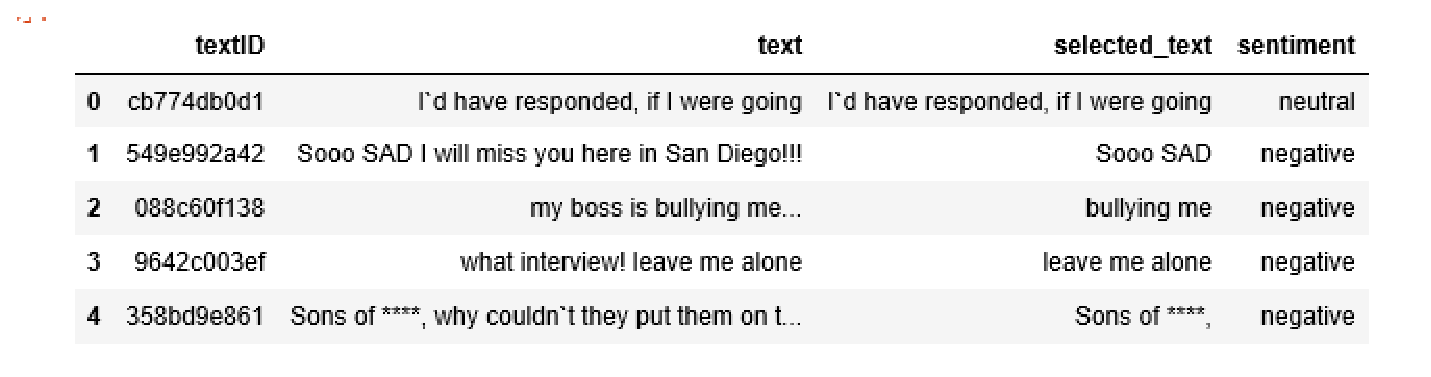
\includegraphics[width=1\textwidth]{kaggle/01.1.eps}
  \caption{}
\end{figure}




%%==========================================================================================
\begin{note}
Let me introduce two existing methods:
Feature selection and score-and-search.

For feature selection,
the query point can be regarded as positive class and
the rest of the data can be regarded as negative class,
selected the features that best distinguish the two classes.

The advantages of this method are easy to operate,
and it's able to resolve dimensionality bias.
However, it has some drawbacks.
Firstly,
positive and negative classes are Not balanced,
secondly,
it can't quantify the outlying degree correctly.
Most importantly,
it doesn't identify group outlying aspects.
\end{note}
%%==========================================================================================

\end{slide}
%%
%%==========================================================================================

%%
%%==========================================================================================
\begin{slide}{Feature Item}
  As you can see from the table above, the four feature
  items in the training set are textID, Text, and selected_text sentiment.
  ~\\
  ~\\
  \bigskip
  \begin{itemize}
    \item textID
    \begin{itemize}
      \item Write the ID of the comment.
    \end{itemize}
    \item Text
    \begin{itemize}
      \item The specific content of the comment.
    \end{itemize}
    \item Selected_text
    \begin{itemize}
      \item Are the keywords that we have chosen to 
      judge the emotional state of the comment.
    \end{itemize}
    \item Sentiment
    \begin{itemize}
      \item The emotional polarity of the sentence.
    \end{itemize}
  \end{itemize}
\end{slide}

%%
%%==========================================================================================
\begin{slide}{Features Item}
  \begin{figure}
    \centering
    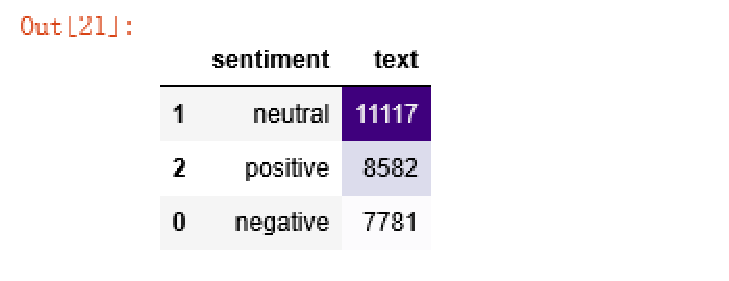
\includegraphics[width=1\textwidth]{kaggle/01.3.eps}
  \end{figure}
  
  \bigskip
  There are three types of sentence emotional polarity.Neurtal
   indicates that the sentence is emotionally neutral, positive
    means the comment is positive, and negative means the 
    comment is negative.
\end{slide}
%%
%%==================================================================



%%==========================================================================================

\section{Constructing Dataset Generator}

%%==========================================================================================
%%

%%
%%===========================================================================================

\begin{slide}{Constructing Dataset Generator}
  Build a dataset generator to analyze each sentence in a comment.
  \begin{itemize}
    \item Input_ids: The id number of each word in the dictionary .
    \item Attention_mask: Which words can be used in the sentence.
    \item Input_type_ids: Distinguish between the preceding sentence 
    and the following sentence.
    \item Target_start: The beginning position in selected_text.
    \item Offsets: Mark the offsets of each word after the participle.
    \item Target_end: End position in selected_text.
    \item Tweet: The original sentence.
    \item Selected_text: Emotional sentences.
    \item Sentiment: The emotional polarity of this sentence.
  \end{itemize}
\end{slide}

%%
%%========================================================================================================


%%
%%===============================================================================================



\section{Modeling}
%%
%%=============================================================================================
\begin{slide}[toc=,bm=]{Build tokenizer to generate the dictionary}
  Because text needs to be processed before natural language processing can take place.
  So we need to turn text into a computer-friendly language. The Tokenizer
   class is used to count the words in the text and generate a document dictionary 
   to support vector representations of the generated text based on the lexicon order.

The 2,323 copies are duplicates and we need to delete them.
We will also evaluate the position of the data points using the coordinates.
%%==========================================================================================
\begin{note}
In conclusion,
we firstly formalized the problem of
group outlying aspects mining,

Then proposed a novel method GOAM algorithm to address the problem of
group outlying aspects mining,
and the proposed method use pruning to reduce time complexity
while identifying the suitable set of outlying features for the interested group.

Thank you and any question?
\end{note}
%%==========================================================================================

\end{slide}
%%
%%==========================================================================================


%%===========================================================================================



%%
%%========================================================================



%%
%%%%===============================================================

%%
%%===================================================================





%%
%%=========================================================================

%%
%%==========================================================================



%%
%%==============================================================================




% TODO: Contact Page

\end{document}

\endinput
